\documentclass[11pt]{article}
\usepackage{booktabs}
\usepackage{color}
\usepackage{rotating}
\usepackage{ifthen}
\usepackage{enumerate}
\usepackage{lscape}
\usepackage{graphicx}

\usepackage[margin=1.3in]{geometry}
\usepackage{tikz}
\newcommand*\circled[1]{\tikz[baseline=(char.base)]{
  \node[shape=circle,draw,inner sep=2pt] (char) {#1};}}

\definecolor{webgreen}{rgb}{0,.5,0}
\definecolor{webbrown}{rgb}{.6,0,0}
\usepackage[colorlinks=true,linkcolor=webgreen,filecolor=webbrown,citecolor=webgreen]{hyperref}

\title{CS 410 Medium-stakes Assignment 3: Writing SQL Queries}
\author{Nick Alexander}
\date{March 30, 2015}

\begin{document}
\maketitle
\vspace*{-0.25in}
\thispagestyle{empty}
\tableofcontents
\newpage


\section{SQL Queries} \label{sec:queries}

In addition to the SQL queries, also show the results retrieved from the PostgreSQL database. You may want to use \verb+\begin{verbatim}+ and \verb+\end{verbatim}+ environment and include the SQL query and retrieved results between \verb+\begin{verbatim}+ and \verb+\end{verbatim}+.

\begin{enumerate}

\item Retrieve all information about courses.

\begin{verbatim}
SELECT *
FROM COURSE
\end{verbatim}

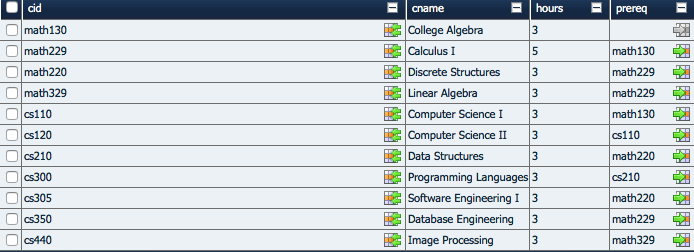
\includegraphics[scale=0.5]{1.png}

\item Retrieve section id, course id, year, and term information for all sections.

\begin{verbatim}
SELECT secid, cid, year, term
FROM SECTION
\end{verbatim}

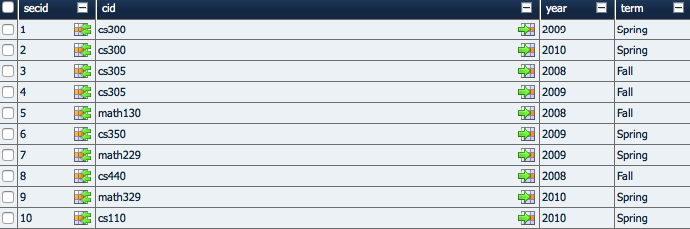
\includegraphics[scale=0.5]{2.png}

\item Retrieve organization id and organization name for all organizations. Rename organization id as ``Organization Code" and organization name as ``Organization Title" in the result set.

\begin{verbatim}
SELECT oid AS "Organization Code", oname AS "Organization Name"
FROM ORG
\end{verbatim}

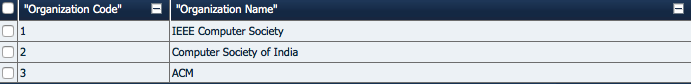
\includegraphics[scale=0.5]{3.png}

\item List course name of courses that are either 2.0 credit hours or 5.0 credit hours.

\begin{verbatim}
SELECT cname
FROM COURSE
WHERE hours=2.0 OR hours=5.0
\end{verbatim}

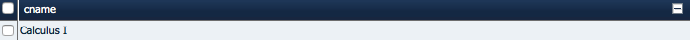
\includegraphics[scale=0.5]{4.png}
 
\item List course name of courses that are not 5.0 credit hours.

\begin{verbatim}
SELECT cname
FROM COURSE
WHERE NOT hours=5.0
\end{verbatim}

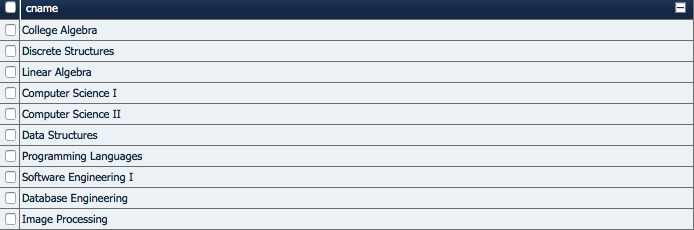
\includegraphics[scale=0.5]{5.png}

\item List course name of courses whose credit  hours are greater than or equal to 2.0 and less than or equal to 4.0.

\begin{verbatim}
SELECT cname
FROM COURSE
WHERE hours>=2.0 AND hours<=4.0
\end{verbatim}

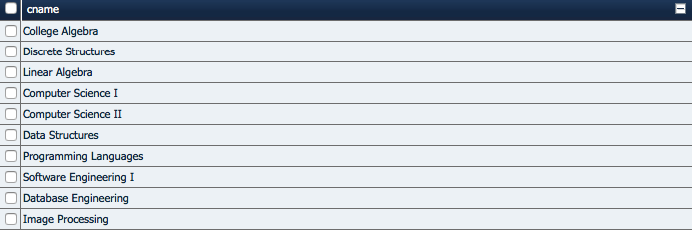
\includegraphics[scale=0.5]{6.png}

\item List organization name whose annual fee is less than \$30.0.

\begin{verbatim}
SELECT oname
FROM ORG
WHERE fee<30.0
\end{verbatim}

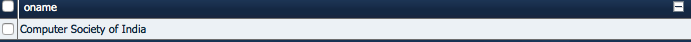
\includegraphics[scale=0.5]{7.png}

\item List organization id and organization name of organizations that charge more than \$50.0 for annual membership fees.

\begin{verbatim}
SELECT oid, oname
FROM ORG
WHERE fee>50.0
\end{verbatim}

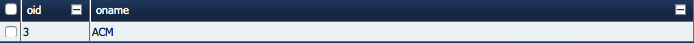
\includegraphics[scale=0.5]{8.png}

\item List course id, course name, and credit hours for courses for which math229 is prerequisite.

\begin{verbatim}
SELECT cid, cname, hours
FROM COURSE
WHERE prereq='math229'
\end{verbatim}

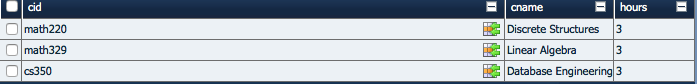
\includegraphics[scale=0.5]{9.png}

\item List student id and student name for all students. Concatenate fist name and last name with a space in between them and show this name under column titled as Name in the result set.

\begin{verbatim}
SELECT fname || ' ' || lname AS Name
FROM STUDENT
\end{verbatim}

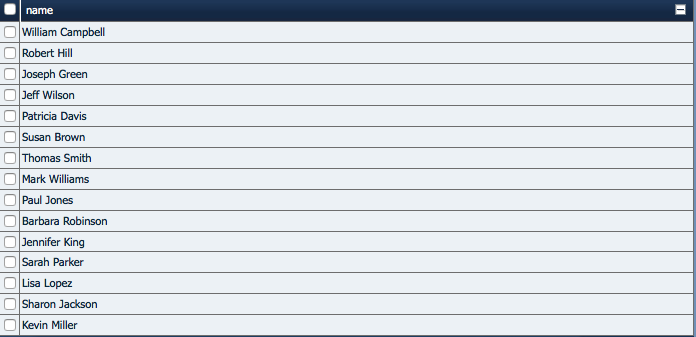
\includegraphics[scale=0.5]{10.png}

\item List course ids of courses that were offered at least once.

\begin{verbatim}
SELECT cid
FROM SECTION
\end{verbatim}

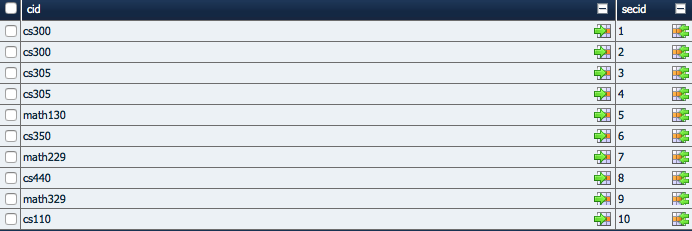
\includegraphics[scale=0.5]{11.png}

\item List distinct courses ids of courses that were offered at least once.

\begin{verbatim}
SELECT DISTINCT cid
FROM SECTION
\end{verbatim}

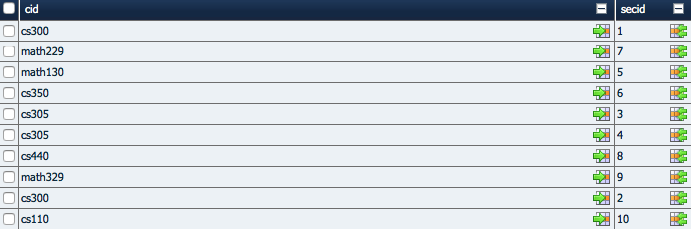
\includegraphics[scale=0.5]{12.png}

\item List course id, year, term, and days for courses that were offered at 11.00 A.M.

\begin{verbatim}
SELECT cid, year, term, days
FROM SECTION
WHERE EXTRACT(HOUR FROM stime)=11
\end{verbatim}

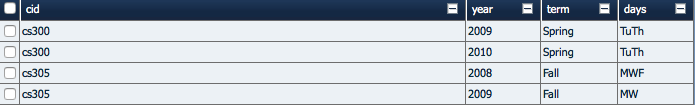
\includegraphics[scale=0.5]{13.png}

\item List course id for courses whose class meeting time ends at 4.45 P.M.

\begin{verbatim}

SELECT cid
FROM SECTION
WHERE EXTRACT(HOUR FROM etime)=16 AND EXTRACT(MINUTE FROM etime)=45

\end{verbatim}

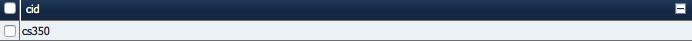
\includegraphics[scale=0.5]{14.png}

\item List all information about courses sorted in decreasing order on course name.

\begin{verbatim}

SELECT *
FROM COURSE
ORDER BY cname ASC;

\end{verbatim}

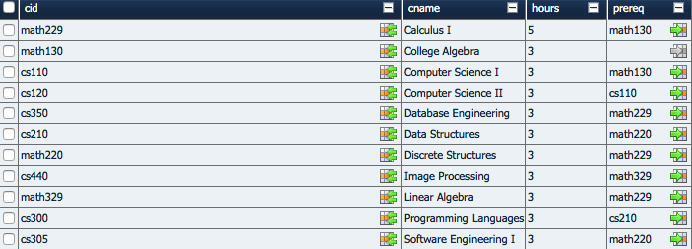
\includegraphics[scale=0.5]{15.png}

\item List all information about section, first sorted in increasing order on year and then in decreasing order on term.

\begin{verbatim}

SELECT *
FROM (
    SELECT *
    FROM SECTION
    ORDER BY term DESC
) AS TMP
ORDER BY year ASC;

\end{verbatim}

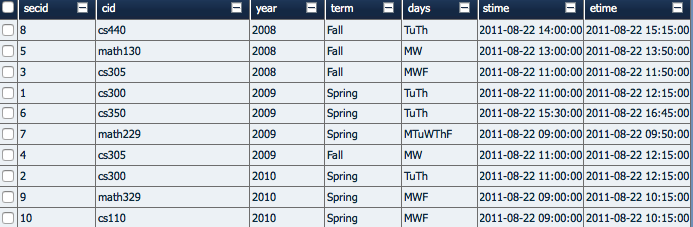
\includegraphics[scale=0.5]{16.png}

\item List course id and course name for courses that don't have prerequisites.

\begin{verbatim}

SELECT cid, cname
FROM COURSE
WHERE prereq IS NULL

\end{verbatim}

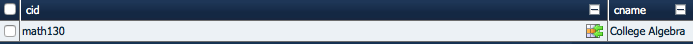
\includegraphics[scale=0.5]{17.png}

\item List course id and course name for courses that have prerequisites.

\begin{verbatim}

SELECT cid, cname
FROM COURSE
WHERE prereq IS NOT NULL

\end{verbatim}

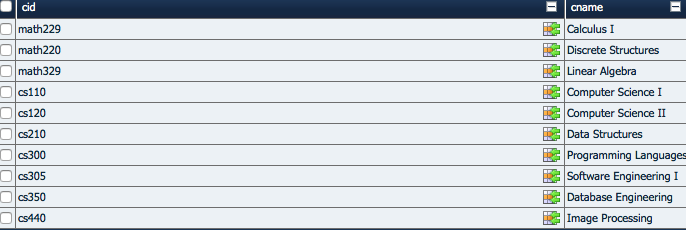
\includegraphics[scale=0.5]{18.png}

\item List name, credit hours, and prerequisite for courses which are either five credit hours, OR course name begins with the letter 'D' and has math229 as prerequisite:

\begin{verbatim}

SELECT cname, hours, prereq
FROM COURSE
WHERE hours=5 OR (SUBSTRING(cname,1, 1)='D' AND prereq='math229')

\end{verbatim}

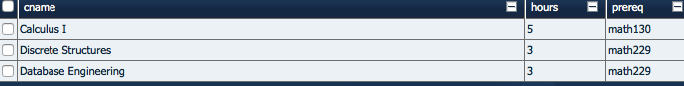
\includegraphics[scale=0.5]{19.png}

\item Retrieve the names of students whose last name ends with the letter `n'.

\begin{verbatim}

SELECT (fname || ' ' || lname) AS Name
FROM STUDENT
WHERE SUBSTRING(lname, LENGTH(lname), 1)='n'

\end{verbatim}

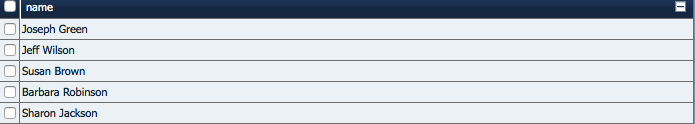
\includegraphics[scale=0.5]{20.png}

\item Retrieve first name of students whose first name begins with the letter 'S', followed by any two characters, followed by the letter `a', and followed by any number of characters.

\begin{verbatim}

SELECT fname
FROM STUDENT
WHERE fname LIKE 'S__a%'
\end{verbatim}

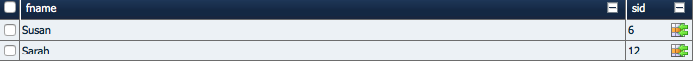
\includegraphics[scale=0.5]{21.png}

\item What is the highest membership fee charged by any organization?

\begin{verbatim}

SELECT MAX(fee)
FROM ORG

\end{verbatim}

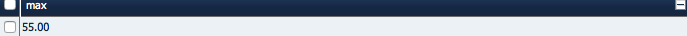
\includegraphics[scale=0.5]{22.png}

\item What is the lowest membership fee charged by any organization?

\begin{verbatim}

SELECT MIN(fee)
FROM ORG

\end{verbatim}

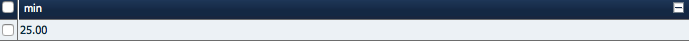
\includegraphics[scale=0.5]{23.png}

\item What is the average membership fee across all organizations?

\begin{verbatim}

SELECT AVG(fee)
FROM ORG

\end{verbatim}

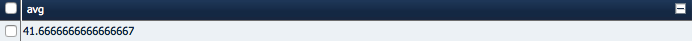
\includegraphics[scale=0.5]{24.png}

\item Let us say that you wanted to become member of all organization. How much money do you need for membership fee?

\begin{verbatim}

SELECT SUM(fee)
FROM ORG

\end{verbatim}

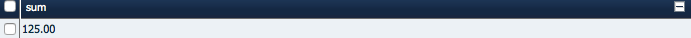
\includegraphics[scale=0.5]{25.png}

\item List section id and course id for courses that begin after 1.00 PM.

\begin{verbatim}

SELECT secid, cid
FROM SECTION
WHERE EXTRACT(HOUR FROM stime)>13

\end{verbatim}

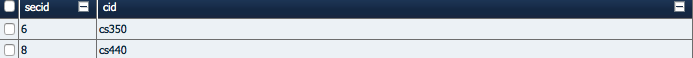
\includegraphics[scale=0.5]{26.png}

\item List section id and course id of courses that end some time between 12:00 noon and 1.00 PM.

\begin{verbatim}

SELECT secid, cid
FROM SECTION
WHERE EXTRACT(HOUR FROM etime)>=12 AND EXTRACT(HOUR FROM etime)<=13

\end{verbatim}

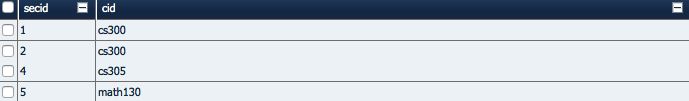
\includegraphics[scale=0.5]{27.png}

\item For each organization, list organization id and its membership count (i.e., the number of people who are members of the organization).

\begin{verbatim}

SELECT oid, COUNT(sid)
FROM MEMBERSHIP
GROUP BY oid

\end{verbatim}

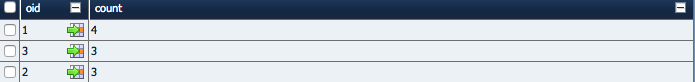
\includegraphics[scale=0.5]{28.png}

\item For those organizations with a membership count of more than three, list organization id and membership count.

\begin{verbatim}

SELECT oid, members
FROM (
     SELECT oid, COUNT(sid)AS members 
     FROM MEMBERSHIP
     GROUP BY oid
) AS TMP
WHERE members>3

\end{verbatim}

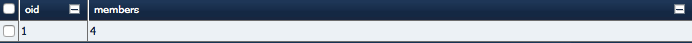
\includegraphics[scale=0.5]{29.png}

\item For each offering of the course named ``Programming Languages," list section id, year, and term.

\begin{verbatim}

SELECT secid, year, term
FROM SECTION, COURSE
WHERE COURSE.cname='Programming Languages'

\end{verbatim}

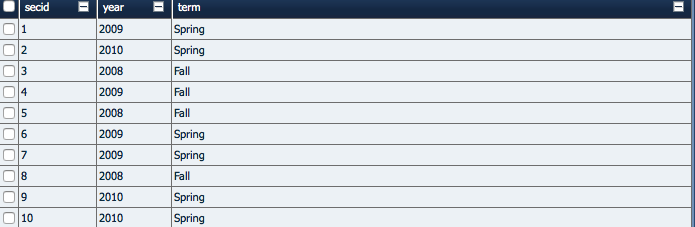
\includegraphics[scale=0.5]{30.png}

\item List all possible combinations of course and section tables. Examine the result set. Are all the rows in the result set meaningful?

\begin{verbatim}

SELECT *
FROM COURSE CROSS JOIN SECTION

\end{verbatim}

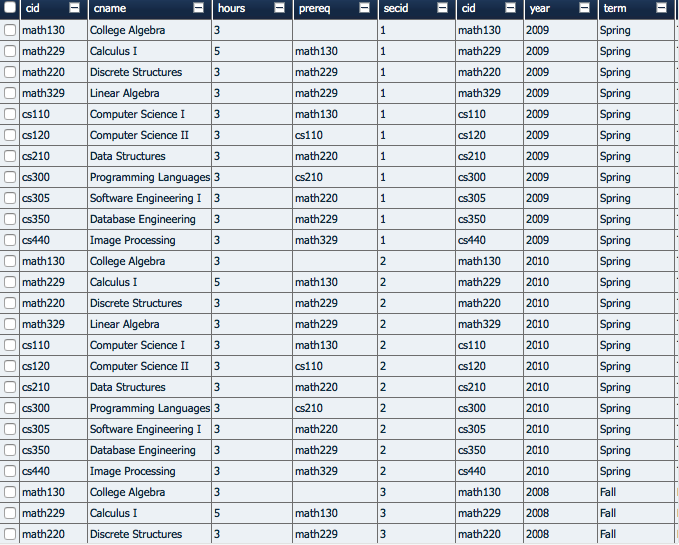
\includegraphics[scale=0.5]{31a.png}\\
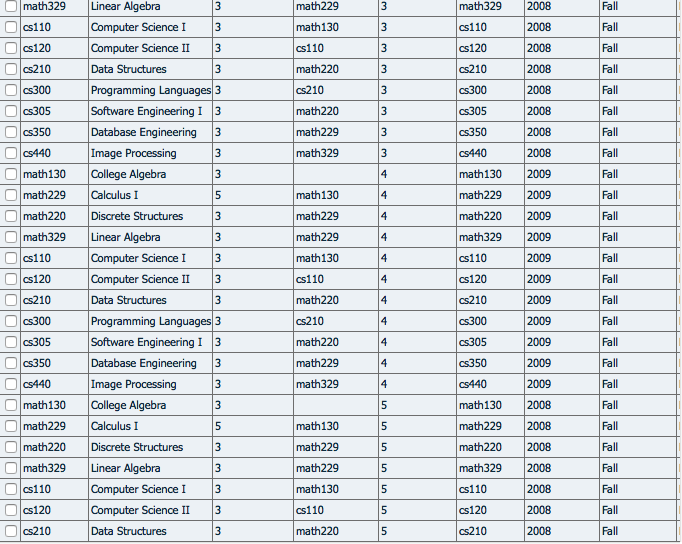
\includegraphics[scale=0.5]{31b.png}\\
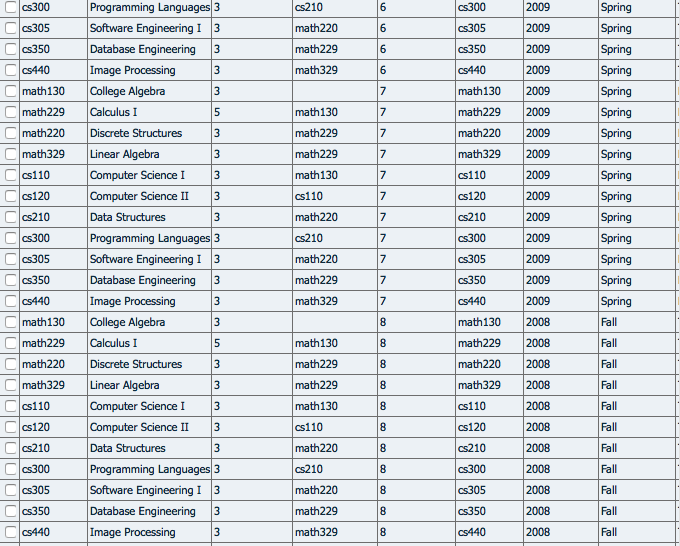
\includegraphics[scale=0.5]{31c.png}\\
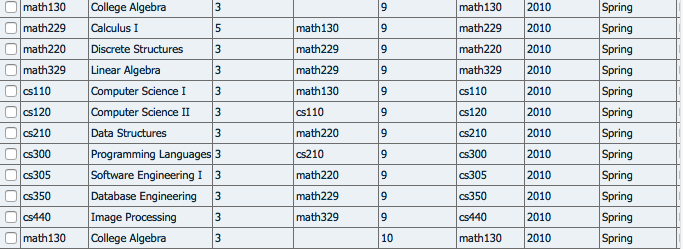
\includegraphics[scale=0.5]{31d.png}

\item How many rows are there in all possible combinations of course and section tables.

\begin{verbatim}

SELECT COUNT(*)
FROM COURSE CROSS JOIN SECTION

\end{verbatim}

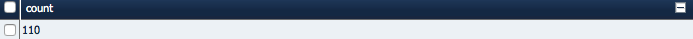
\includegraphics[scale=0.5]{32.png}

\item For students who are members of organizations, list student id and name (first and last), and the names of the organizations.

\begin{verbatim}

Your answer goes here.

\end{verbatim}

\item List student id and name (first and last) for all students, and if they have enrolled in any sections, list section id and grade for each section.

\begin{verbatim}

SELECT STUDENT.sid, fname || ' ' || lname AS name, secid, grade
FROM STUDENT, ENROLLMENT
WHERE STUDENT.sid=ENROLLMENT.sid

\end{verbatim}

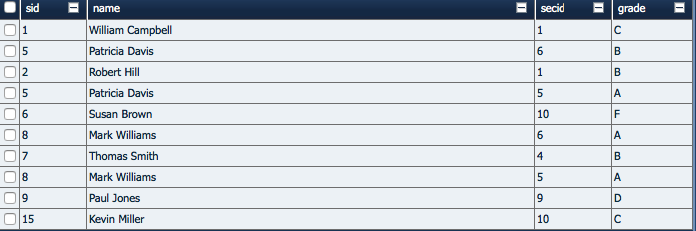
\includegraphics[scale=0.5]{34.png}

\item List student id and name (first and last) of all students, as well as the names of organizations if they happen to be members.

\begin{verbatim}

SELECT STUDENT.sid, fname, lname, oname
FROM STUDENT, MEMBERSHIP, ORG
WHERE STUDENT.sid=MEMBERSHIP.sid AND MEMBERSHIP.oid=ORG.oid
ORDER BY STUDENT.sid

\end{verbatim}

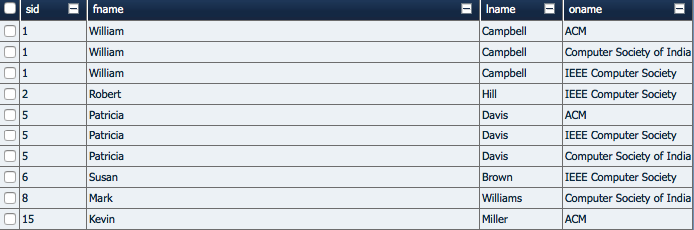
\includegraphics[scale=0.5]{35.png}

\item For courses that have prerequisites, list course id, course name, prerequisite course id, and prerequisite course name.

\begin{verbatim}

SELECT DISTINCT cname
FROM course c, (SELECT prereq
      FROM course) as temp
WHERE c.cid = temp.prereq

\end{verbatim}

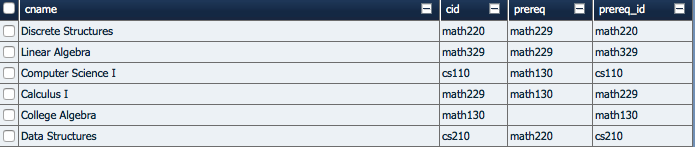
\includegraphics[scale=0.5]{36.png}

\item List course id, course name, prerequisite course name (if any) for all courses.

\begin{verbatim}

Your answer goes here.

\end{verbatim}

\item For students pursuing degree programs, list student id and the name of the degree program.

\begin{verbatim}

SELECT STUDENT.sid, DEGREE.dname
FROM STUDENT, MAJOR, DEGREE
WHERE STUDENT.sid=MAJOR.sid AND MAJOR.dcode=DEGREE.dcode

\end{verbatim}

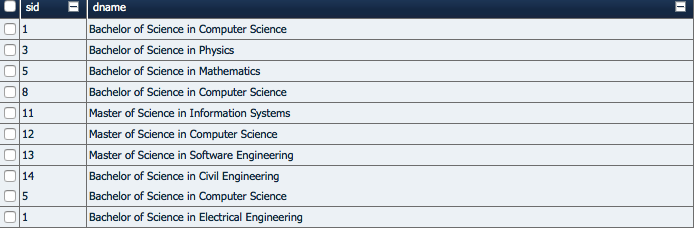
\includegraphics[scale=0.5]{38.png}

\item For each student, list last name and the name(s) of degree programs the student is majoring in, sorted by student last name.

\begin{verbatim}

SELECT STUDENT.lname, DEGREE.dname
FROM STUDENT, DEGREE, MAJOR
WHERE STUDENT.sid=MAJOR.sid AND MAJOR.dcode=DEGREE.dcode
ORDER BY STUDENT.lname

\end{verbatim}

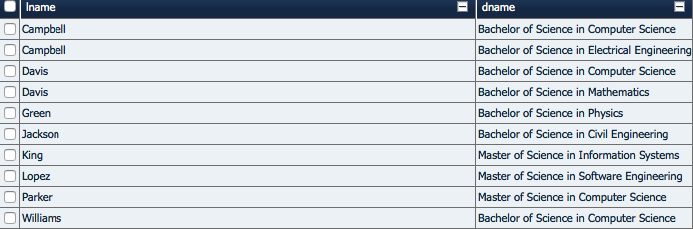
\includegraphics[scale=0.5]{39.png}

\item List last names of students who are either enrolled in at least one degree program or members of some organization.

\begin{verbatim}

SELECT DISTINCT STUDENT.fname, STUDENT.lname
FROM STUDENT, MAJOR, MEMBERSHIP
WHERE STUDENT.sid=MAJOR.sid OR STUDENT.sid=MEMBERSHIP.sid

\end{verbatim}

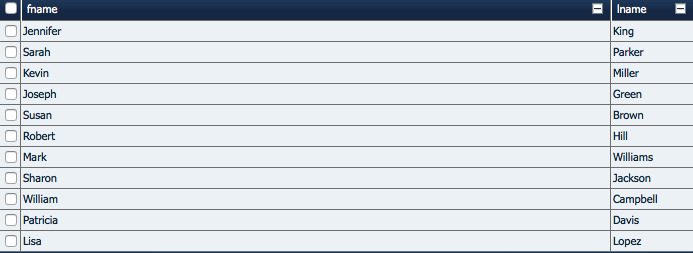
\includegraphics[scale=0.5]{40.png}

\item List last names of students who are either enrolled in at least one degree program \emph{or} members of some organization. Don't remove duplicate last names.

\begin{verbatim}

Your answer goes here.

\end{verbatim}


\item List last names of students who are enrolled in at least one degree program \emph{and} are also members of some organization.

\begin{verbatim}

SELECT fname, lname
FROM (
    SELECT sid
    FROM MAJOR
    INTERSECT
    SELECT sid
    FROM MEMBERSHIP
) AS TMP, STUDENT
WHERE STUDENT.sid=TMP.sid

\end{verbatim}

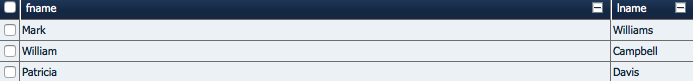
\includegraphics[scale=0.5]{42.png}

\item List last names of students who are enrolled in at least one degree program but are not members of any organization.

\begin{verbatim}

SELECT fname, lname
FROM (
    SELECT sid
    FROM MAJOR
    EXCEPT
    SELECT sid
    FROM MEMBERSHIP
) AS TMP, STUDENT
WHERE STUDENT.sid=TMP.sid

\end{verbatim}

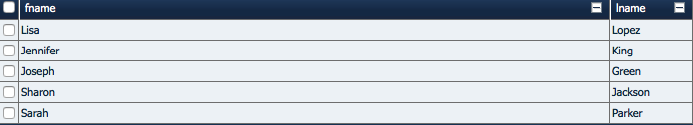
\includegraphics[scale=0.5]{43.png}

\item List student id and last name of all students, as well as the name(s) of degree programs that they are pursuing (if any). The result set should also show the names of degree programs even if no student is pursuing such degree programs.

\begin{verbatim}

SELECT sid, lname, dname
FROM (

    SELECT STUDENT.sid, STUDENT.lname, MAJOR.dcode
    FROM STUDENT, MAJOR
    WHERE STUDENT.sid=MAJOR.sid
) AS TMP
RIGHT OUTER JOIN DEGREE
ON TMP.dcode=DEGREE.dcode


\end{verbatim}

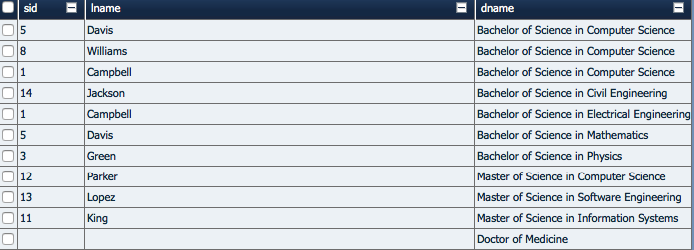
\includegraphics[scale=0.5]{44.png}

\item For courses that have been offered one or more times, list course name, section id, and year.

\begin{verbatim}

SELECT COURSE.cname, SECTION.secid, SECTION.year
FROM (
    SELECT COUNT(*) AS offerings, cid
    FROM SECTION
    GROUP BY cid
) AS TMP, SECTION, COURSE
WHERE TMP.offerings>1 AND COURSE.cid=SECTION.cid
ORDER BY SECTION.year

\end{verbatim}

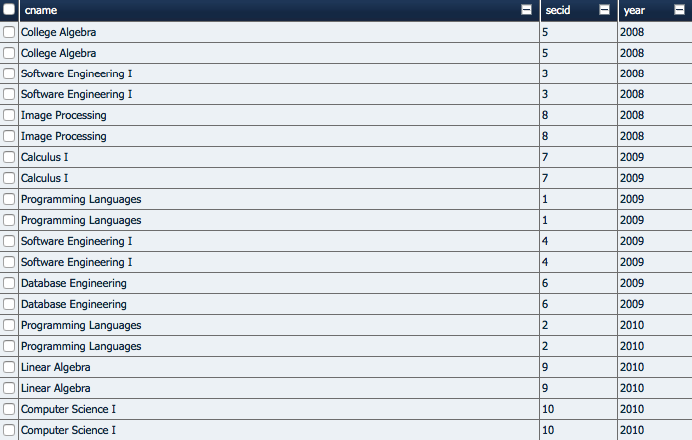
\includegraphics[scale=0.5]{45.png}

\item List name and fee of organizations whose membership fee is greater than the average membership fee across all organizations.

\begin{verbatim}

SELECT ORG.oname, ORG.fee
FROM (
     SELECT AVG(fee) AS avg_fee
     FROM ORG
) as TMP, ORG
WHERE ORG.FEE>TMP.avg_fee

\end{verbatim}

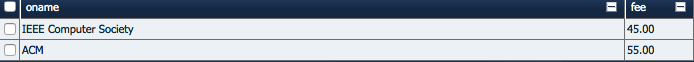
\includegraphics[scale=0.5]{46.png}

\item List course id and course name for courses that have never been offered.

\begin{verbatim}

SELECT cid
FROM COURSE
EXCEPT
SELECT cid
FROM SECTION

\end{verbatim}

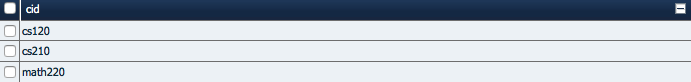
\includegraphics[scale=0.5]{47.png}

\item List course id and course name for courses that have been offered at least once.

\begin{verbatim}

SELECT cid, cname
FROM COURSE
WHERE EXISTS (
    SELECT cid
    FROM SECTION
)

\end{verbatim}

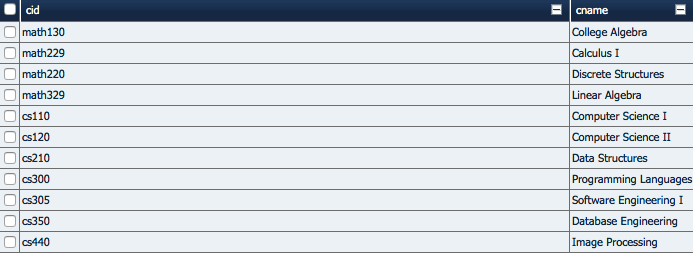
\includegraphics[scale=0.5]{48.png}

\item For students who have taken courses (i.e., enrolled in sections), list student id and last name, as well as course id, course name, year, term, and grade for each course. Use natural join.

\begin{verbatim}

SELECT STUDENT.sid, STUDENT.lname, COURSE.cname, SECTION.cid, SECTION.term, SECTION.year, ENROLLMENT.grade
FROM STUDENT, ENROLLMENT, COURSE, SECTION
WHERE STUDENT.sid=ENROLLMENT.sid AND ENROLLMENT.secid=SECTION.secid AND COURSE.cid=SECTION.cid

\end{verbatim}

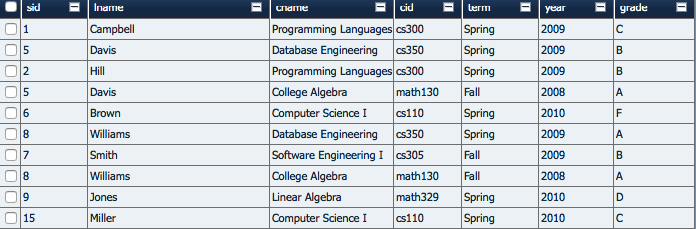
\includegraphics[scale=0.5]{49.png}

\item For students who have taken courses (i.e., enrolled in sections), list student id and last name, as well as course id, course name, year, term, and grade for each course. The result set should also include a new column at the very end titled ``Remarks." If the student has earned an `A', Remarks column should display Superior. Likewise, Good for a `B', Average for `C', Poor for `D', Incomplete for `I', Fail for `F', and Withdrawn for `W.'

\begin{verbatim}

Your answer goes here.

\end{verbatim}


\end{enumerate}


\section{Preparing Written Report}

Use the \LaTeX{}\ template to generate your solution in PDF format.


\begin{landscape}

\section{Rubric} \label{sec:Rubric}

Use the following rubric to evaluate your response to this assignment.

\vspace*{0.15in}

\begin{tabular}{p{1.2in}p{1.5in}p{1.5in}p{1.5in}p{1.5in}} \toprule
\multicolumn{1}{r}{\emph{Perf Level}} & \multicolumn{1}{c}{\emph{Outstanding}} & \multicolumn{1}{c}{\emph{Good}} & \multicolumn{1}{c}{\emph{Fair}} & \multicolumn{1}{c}{\emph{Poor}} \\ 
\multicolumn{1}{c}{\emph{Trait}} & & & & \\ \midrule

\emph{Problem Analysis} &
Precise and concise documentation to support the claim that the problem is correctly and thoroughly analyzed prior to writing the query is provided. &
Sufficient documentation, though verbose and non-coherent, to support the claim that the problem is correctly analyzed prior to writing the query is provided. &
Some documentation to support the claim that the problem is superficially analyzed prior to writing the query is provided. &
Documentation to support the claim that the problem is analyzed prior to writing the query is not provided. \\ \midrule


\emph{Query Execution} & 
The query compiles and produces correct results. Also, the query runs efficiently. & 
Though inefficient, the query compiles and produces correct results. &
The query compiles but produces incorrect results. &
The query does not compile. \\ \midrule

\emph{Correctness Arguments} & 
The correctness of the query is argued using rigorous statements. &
The correctness of the query is argued using informal logical statements. &
The correctness of the query is argued using illogical  statements. &
There are no statement about the query correctness. \\ \midrule


\emph{Completeness} &
Answers to all questions in the assignment are provided. Queries compile and run. Problem analysis documentation and correctness arguments are provided. &
Answers to less than 75\% of the questions in the assignment are provided. Queries compile and run. Problem analysis documentation and correctness arguments are provided. &
Answers to less than 50\% of the questions in the assignment are provided. Queries compile and run. Problem analysis documentation and correctness arguments are provided. &
Answers to less than 25\% of the questions in the assignment are provided. Queries compile and run. Problem analysis documentation and correctness arguments are provided. \\ \bottomrule

\end{tabular}


\end{landscape}

\section{Self-assessment}

Use the following table and the rubric of section~\ref{sec:Rubric} to score your solution. Circle the appropriate number in each row. For example, to circle 20, use the \LaTeX{} markup code \verb+\circled{20}+, which produces \circled{20}.

\vspace*{0.2in}

\begin{tabular}{lcccc} \\ \toprule
\multicolumn{1}{r}{\emph{Perf Level}} & \emph{Outstanding} & \emph{Good} & \emph{Fair} & \emph{Poor} \\ 
\emph{Trait} & & & & \\ \toprule

\emph{Problem Analysis} &  \circled{10}  &  8  &  6  & 4 \\ \midrule


\emph{Query Execution} &  \circled{30} & 25 & 20 & 15 \\ \midrule


\emph{Correctness Arguments} &  \circled{10} & 8 & 6 & 4 \\ \midrule


\emph{Completeness} &  \circled{50}  &  40 & 30  &  20 \\ \bottomrule

\end{tabular}


\end{document}
